\section{Návrh uživatelského rozhraní - Hi-Fi prototyp}

Dalším krokem návrhu uživatelského rozhraní byla tvorba Hi-Fi prototypu, neboli aplikace, která je již vytvořena za použití některých technologií cílové platformy, avšak neobsahuje backend - neukládá žádná data a vždy zobrazuje pouze předpřipravený obsah - vždy však musí správně reagovat na interakci uživatele.\\
Hi-Fi prototyp jsme stále realizovali jako tým v rámci předmětu MI-NUR, avšak přípravu technologie jsem provedl já samostatně a její realizace stojí za zmínku.

%%%%%%%%%%%%%%%%%%%%%%%%%%%%%%%%%%%%%%%%
%%%%%%%%%%%%%%%%%%%%%%%%%%%%%%%%%%%%%%%%

\subsection{Technologie použitá v Hi-Fi prototypu}

Cílem bylo vytvořit jakýsi mikro-framework, ve kterém bude snadné tvořit \mbox{Hi-Fi} prototyp a současně bude možné používat standardní prvky Material designu. Kód měl být psán v jazyce cílové platformy, tedy HTML + CSS + JS.\\
Jelikož nikdo z nás neměl zkušenosti s žádným z javascriptových frameworků typu Angular či React a já jsem chtěl pro naše řešení mít co nejméně závislostí, rozhodl jsem se vše napsat v čistém Javascriptu (pouze za použití dnes de facto standardní knihovny jQuery, která se dá jednoduše načíst z CDN). Základem je jeden výchozí HTML soubor, viz ukázka kódu \ref{code:hifi-html}.

\begin{listing}[H]
\begin{minted}[linenos,frame=lines]{html}
<!DOCTYPE html>
<html>
<head>
  <title>SYSEL</title>

  <meta name="viewport" content="width=device-width, initial-scale=1.0">
  <meta charset="UTF-8">

  <!-- Material components all-in-one -->
  <link rel="stylesheet" type="text/css" href="https://unpkg.com/
  material-components-web@latest/dist/material-components-web.min.css"/>
</head>
<body>
  <div id="main-content" class="homepage-include"></div>

  <!-- Material design -->
  <script src="https://unpkg.com/material-components-web@latest/dist/
  material-components-web.min.js"></script>
  <!-- jQuery-->
  <script src="https://cdnjs.cloudflare.com/ajax/libs/jquery/
  2.2.4/jquery.min.js"></script>
  <!-- Custom scripts -->
  <script src="js/main.js"></script>
</body>
</html>
\end{minted}
\caption{Základní soubor index.html pro Hi-Fi prototyp} \label{code:hifi-html}
\end{listing}

Veškerý ostatní obsah je \emph{komponenta}, což je HTML šablona, která může být libovolně vkládána do jiných šablon, několikrát vedle sebe apod. Postupně jsem umožnil komponenty libovolně parametrizovat a samozřejmě je mezi sebou vyměňovat - například přechod na zcela jinou stránku je realizován přes \emph{výměnu komponenty}, která se zobrazuje v \code{\#main-content} v ukázce kódu \ref{code:hifi-html}.\\
Toto vše je možné díky pouhým 67 řádkům JS kódu. Úryvek je vidět v ukázce kódu \ref{code:hifi-js}.

\begin{listing}[H]
\begin{minted}[linenos,frame=lines]{javascript}
function loadDynamicContent(selector = '[class$="-include"]', callback){

  $(selector).each(function (e) {
    // load all custom components
    let parent = $(this);
    $(this).html('');
    $(this).load("components/" + $(this).attr("class")
      .replace("-include", "") +  ".html", function() {

      // load sub-components
      $(this).find('[class$="-include"]').each(function() {
        loadDynamicContent(this, function(){
            insertParameters(parent)
        });
      });
      if ($(this).find('[class$="-include"]').length === 0) {
        insertParameters(parent);
      }
      callback(this);
    });
  });
}

function insertParameters(parent) {
    let parameters = parent.attr('data-include-content');
    if (parameters !== undefined) {
        $.each(JSON.parse(parameters), function(key, value){
            parent.html(parent.html().replace('{' + key + '}', value));
        }
    }
}
\end{minted}
\caption[Funkce pro načtení obsahu komponent Hi-Fi prototypu]{Funkce pro načtení obsahu komponent Hi-Fi prototypu, včetně podkomponent} \label{code:hifi-js}
\end{listing}

Funkce \code{loadDynamicContent} z ukázky kódu \ref{code:hifi-js} funguje tak, že projde existující kód (výchozí je vždy \code{index} z ukázky kódu \ref{code:hifi-html}) a veškeré výskyty tříd ve tvaru \code{foo-include} nahrazuje obsahem souboru \code{foo.html} ze složky \code{components/}.\\
Díky tomu, že Javascriptu může být umožněn přístup na filesystém, lze takto dynamicky načítat obsah souborů z disku a renderovat ho přímo v již načteném obsahu. Tato technika je v některých browserech zablokována kvůli CORS\footnote{Cross-origin resource sharing - ochrana před načítáním nezabezpečeného obsahu}, a tak pro použití například v Google Chrome je nutné zmiňovaný \code{index} spouštět přes libovolný webserver, nelze jej přímo otevřít z filesystému. Na druhou stranu například v Mozilla Firefoxu je CORS v tomto ohledu volnější, a celý tento mikro-framework tak lze používat bez jakéhokoliv lokálního serveru, stahování závislostí atp. - stačí pouze otevřit \code{index.html}.\\

\subsection{Realizace Hi-Fi prototypu}

Podobně jako přípravu technologie, i některá důležitá rozhodnutí týkající se designu UI jsem navrhoval samostatně bez týmu a budu je proto probírat v textu níže.\\
Kompletní zdrojové kódy prototypu jsou dostupné na přiloženém médiu a také v repozitáři na Gitlab FIT \cite{gitlab-hifi}.\\

\begin{figure}[h]
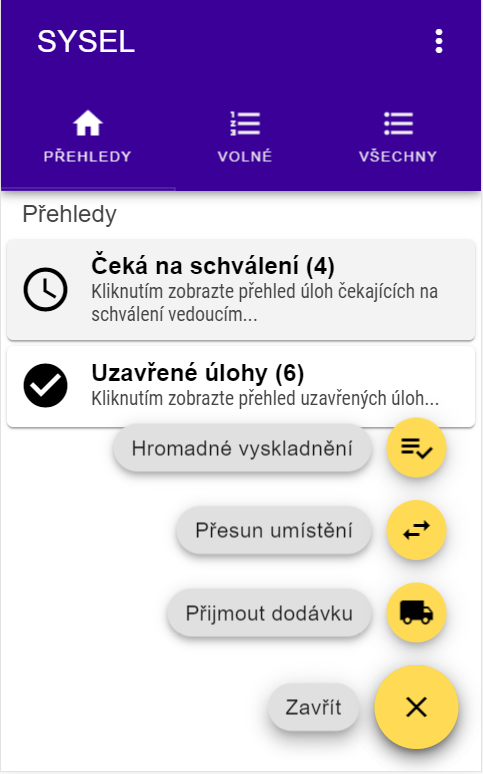
\includegraphics[height=0.45\textheight]{../png/hifi/fab.png}
\caption{Rychlé menu v pravé dolní části obrazovky: Hi-Fi prototyp} \label{picture:hifi:fab}
\end{figure}

\paragraph{Rychlé menu.} Ve druhém prototypu jsem poprvé použil akční tlačítko plovoucí v pravém dolním rohu aplikace, přes které se tvoří nové položky. Je-li na stránce možné tvořit více různých věcí, otevře se z něj menu, jaké známe převážně z Google aplikací - jak je znázorněno na obrázku \ref{picture:hifi:fab}. Toto tlačítko již v aplikaci vydrželo i do reálné verze a jak na něj uživatelé reagovali se dočtete v sekci \ref{sec:usertest}.

\begin{figure}[h]
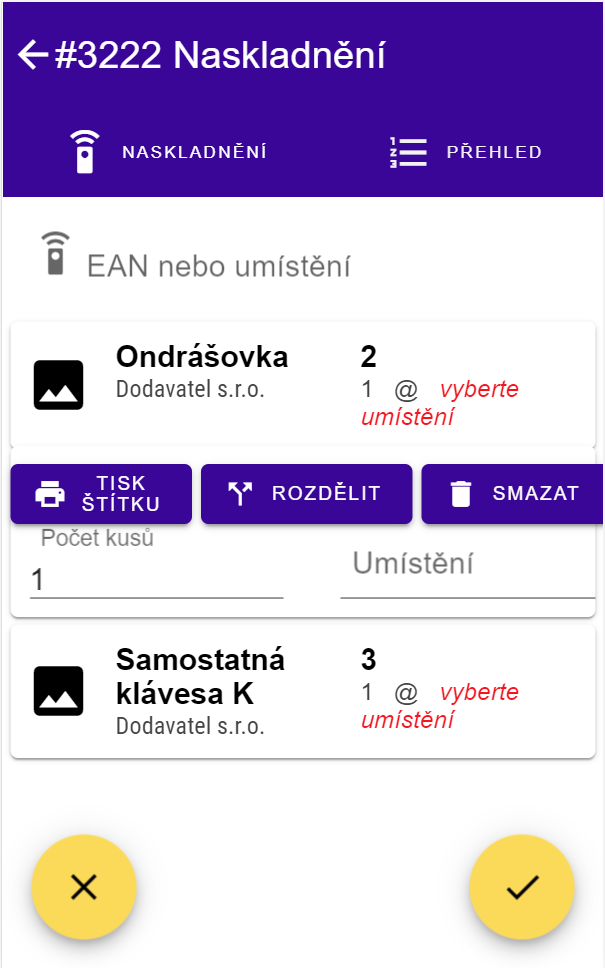
\includegraphics[height=0.5\textheight]{../png/hifi/naskladneni.png}
\caption{Rozhraní skladníka pro naskladňování položek: Hi-Fi prototyp} \label{picture:hifi:naskladneni}
\end{figure}

\begin{figure}[h]
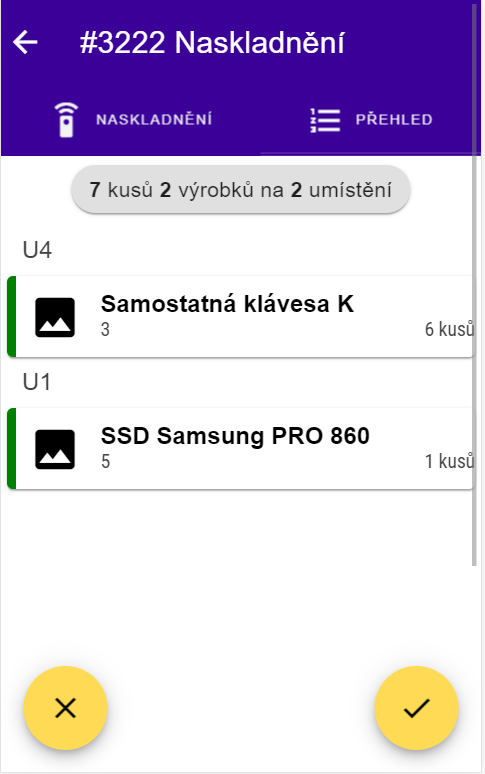
\includegraphics[height=0.5\textheight]{../png/hifi/dokonceni.png}
\caption{Rozhraní skladníka pro naskladňování položek - dokončení: Hi-Fi prototyp} \label{picture:hifi:dokonceni}
\end{figure}

\paragraph{Naskladnění.} Stejně jako u předchozí verze prototypu, i nyní je do textu vložena ukázka obrazovky naskladnění - je to z toho důvodu, že většina úkolů má ve svém nitru obdobný průběh, což vzešlo z analýzy v sekci \ref{sec:analysis}. V této verzi prototypu je však již úkol ve svém detailu rozdělen na dvě obrazovky, mezi kterými je - stejně jako na domovské obrazovce - možné přejet posunutím nebo kliknutím v záhlaví aplikace, čímž je pro uživatele snadnější zobrazit si vždy tu informaci, kterou hledá - v případě úkolu naskladnění se jedná o rozdělení na samotnou realizaci \emph{naskladňování} (obrázek \ref{picture:hifi:naskladneni}) a na \emph{přehled} (obrázek \ref{picture:hifi:dokonceni}). I na tyto obrazovky se dostalo akční tlačítko, navržené pro zobrazení menu, avšak zde mělo funkci dokončení, případně odmítnutí úkolu, což se v uživatelském testování projevilo jako matoucí, a tak byla tato tlačítka - viditelná ve spodní části obrazovek - v reálné aplikaci odstraněna a nahrazena běžnými tlačítky s popisky, která se zobrazují na stránce \emph{přehled}.

%%%%%%%%%%%%%%%%%%%%%%%%%%%%%%%%%%%%%%%%%%%%%%%%%%%%%%%%%%%%%%%%%%%%%%%%%%%%%%%%
%%%%%%%%%%%%%%%%%%%%%%%%%%%%%%%%%%%%%%%%%%%%%%%%%%%%%%%%%%%%%%%%%%%%%%%%%%%%%%%%
%%%%%%%%%%%%%%%%%%%%%%%%%%%%%%%%%%%%%%%%%%%%%%%%%%%%%%%%%%%%%%%%%%%%%%%%%%%%%%%%
%%%%%%%%%%%%%%%%%%%%%%%%%%%%%%%%%%%%%%%%%%%%%%%%%%%%%%%%%%%%%%%%%%%%%%%%%%%%%%%%

\section{Testování Hi-Fi prototypu}

Vzniklý Hi-Fi prototyp byl testován v rámci předmětu MI-NUR společně mnou, Pavlem Kovářem, Martinem Kubišem a Jakubem Šterclem. Abych nevyužíval cizí práci, uvedu v tomto textu pouze části, které jsou realizoval já osobně, práci ostatních kolegů jsem ale zhodnotil v samotné implementaci následné funkční aplikace.

%%%%%%%%%%%%%%%%%%%%%%%%%%%%%%%%%%%%%%%%
%%%%%%%%%%%%%%%%%%%%%%%%%%%%%%%%%%%%%%%%

\subsection{Heuristická analýza}

Zvolili jsme několik akcí skladníka, které jsme podrobili heuristické analýze. Konkrétně já jsem řešil obrazovku naskladnění (screenshoty \ref{picture:hifi:naskladneni} a \ref{picture:hifi:dokonceni}), která dopadla následovně:

\begin{enumerate}
  \item \emph{Viditelnost stavu systému}:\\Vše v pořádku.
  \item \emph{Shoda mezi systémem a realitou}:\\OK.
  \item \emph{Minimální zodpovědnost (a stres)}:\\Při otevření tohoto úkolu je jeho řešitel ihned nastaven na právě přihlášeného uživatele. Pro navrácení je nutné jej stornovat a vyplnit, že se jednalo o chybu. V systému o tom však bude záznam. Dále není jasné, zda tlačítka ve spodní části úkol již odešlou, nebo se teprve zobrazí nějaký formulář a potvrzení.\footnote{V reálné aplikaci je toto vyřešeno: úkol při otevření - pokud ještě není přiřazen - zobrazí pouze informace a tlačítko pro přiřazení úkolu \uv{sám sobě}. Teprve poté je možné v něm provádět práci.}
  \item \emph{Shoda s použitou platformou a obecnými standardy}:\\V pořádku (material design).
  \item \emph{Prevence chyb}:\\Úkol nelze dokončit, pokud některé zboží nemá vyplněno umístění.\footnote{V reálné aplikaci byla kompletně otočena logika označování umístění: nejprve je nutné zvolit umístění, a pak na něj teprve ukládat zboží. Popsaná situace tedy nemůže nastat.} Jiné chyby na této stránce (z aplikačního hlediska) prakticky nelze udělat => OK.
  \item \emph{Kouknu a vidím}:\\Při větším množství položek může být seznam dlouhý a nepřehledný.
  \item \emph{Flexibilita a efektivita}:\\OK - zkušený může stále pípat, nový může zkoumat dostupné vstupy.
  \item \emph{Minimalita (Klapky na očích)}:\\OK - obsah karet bude ve finální aplikaci konfigurovatelný\footnote{V době psaní textu se jedná o jeden z návrhů na budoucí vylepšení aplikace}.
  \item \emph{Smysluplné chybové hlášky}:\\Jediná chybová hláška o vyplnění umístění je jasná.
  \item \emph{Help a dokumentace}:\\Dokumentace není\footnote{Reálná aplikace již základní nápovědu / dokumentaci nabízí}.
\end{enumerate}

%%%%%%%%%%%%%%%%%%%%%%%%%%%%%%%%%%%%%%%%
%%%%%%%%%%%%%%%%%%%%%%%%%%%%%%%%%%%%%%%%

\subsection{Uživatelské testování prototypu}

Hi-Fi prototyp aplikace byl již otestován více potenciálními uživateli, pro které jsme připravili seznam úkolů k řešení. Tyto úkoly prováděli na mobilních zařízeních, avšak bohužel bez podpory čtečky čárových kódů, neboť zařízení se zabudovanou čtečkou jsem měl k dispozici pouze jedno a testování probíhalo na více místech současně. Zmiňovaný seznam úkolů a také výstupy testování těch uživatelů, které jsem testoval já osobně, jsou dostupné v příloze \ref{ap:hifi:test}. Problémy nalezené v prototypu byly buďto řádně opraveny ještě v rámci prototypu, nebo s nimi bylo počítáno při realizaci reálné aplikace.
